\documentclass[tikz, border=5mm]{standalone}
\usepackage{tikz}
\usetikzlibrary{calc, arrows.meta, shapes.geometric, angles, quotes} % Include necessary libraries

\begin{document}
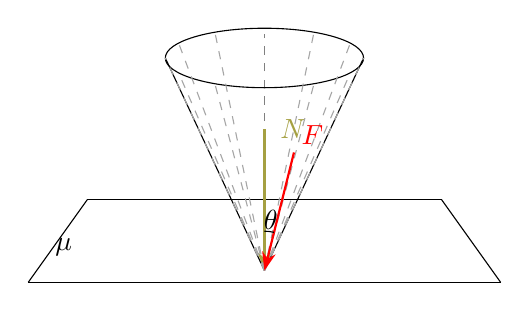
\begin{tikzpicture}[
    scale=1.5, % Adjust overall scale if needed
    >=Stealth, % Use Stealth arrow tips
    force/.style={<-, thick, red}, % Style for the force vector F (changed color)
    normalforce/.style={<-, thick, yellow!60!black}, % Style for the normal force vector N
    axis/.style={-, dashed, gray}, % Style for the normal axis
    cone line/.style={-, black}, % Style for cone boundary lines
    cone fill line/.style={-,dashed, gray!70} % Style for lines indicating cone volume
  ]

  % --- Coordinates ---
  \coordinate (contact) at (0,0); % Contact point (origin)

  % --- Surface ---
  \draw (-2,-0.1) -- (2,-0.1); % Front edge of the surface
  \draw (-1.5,0.6) -- (1.5,0.6); % Back edge of the surface
  \draw (-2,-0.1) -- (-1.5,0.6); % Left edge
  \draw (2,-0.1) -- (1.5,0.6);  % Right edge
  \node at (-1.7, 0.2) {$\mu$}; % Label for friction coefficient

  % --- Normal Axis (Upwards from the surface) ---
  \coordinate (N_axis_end) at (0, 2); % End point of the normal axis visual representation
  \draw[axis] (contact) -- (N_axis_end); % Draw normal axis upwards

  % --- Normal Force Vector N ---
  \coordinate (N_end) at (0, 1.2); % End point of the normal force vector N
  \draw[normalforce] (contact) -- (N_end) node[right=2pt] {$N$}; % Draw normal force vector N

  % --- Friction Cone (Opening upwards) ---
  \def\coneangle{25} % Define the friction angle (alpha) in degrees (adjust for visual appearance)
  \def\conehight{1.8} % Define the visual height of the cone upwards (adjusted height)
  \pgfmathsetmacro{\coneradius}{\conehight*tan(\coneangle)}
  \pgfmathsetmacro{\coneellipseY}{0.3*\coneradius}

  % Cone boundary lines (generators)
  \coordinate (C_left) at ({-\coneradius}, \conehight);
  \coordinate (C_right) at ({\coneradius}, \conehight);
  \draw[cone line] (contact) -- (C_left);
  \draw[cone line] (contact) -- (C_right);

  % Cone base ellipse (perspective view) at the top
  \draw[cone line] ($(contact)+(0,\conehight)$) ellipse ({\coneradius} and {\coneellipseY});

  % Internal lines to suggest the cone's volume
  \foreach \angle in {120, 150, 180, 210, 240} {
      \coordinate (p) at ($(contact)+(0,\conehight) + (\angle:{\coneradius} and {\coneellipseY})$);
      \draw[cone fill line] (contact) -- (p);
  }
   \foreach \angle in {-60, -30, 0, 30, 60} {
      \coordinate (p) at ($(contact)+(0,\conehight) + (\angle:{\coneradius} and {\coneellipseY})$);
      \draw[cone fill line] (contact) -- (p);
  }

  % --- Applied Force F (pointing outwards from contact, within the cone) ---
  % Endpoint chosen to be inside the cone visually
  \coordinate (F_end) at (0.25, 1.0); % Example endpoint for F, inside the cone
  \draw[force] (contact) -- (F_end) node[above right=-1pt] {$F$}; % Draw the force vector F pointing outwards

  % --- Angle theta between N and F ---
  % Define points for angle calculation
  \coordinate (Origin) at (contact);
  \coordinate (Point_N) at (N_end); % Use the endpoint of N vector for angle
  \coordinate (Point_F) at (F_end); % Use the endpoint of F vector for angle

  % Draw the angle arc and label
  \pic [draw, -, "$\theta$", angle eccentricity=1.3, angle radius=0.5cm] {angle = Point_F--Origin--Point_N};

\end{tikzpicture}
\end{document}